\documentclass{article}
\usepackage[utf8]{inputenc}
\usepackage[brazil]{babel}
\usepackage{hyperref}
\usepackage[paper=a4paper,lmargin=1.5cm, rmargin=1.5cm, tmargin=1.6cm, bmargin=1.5cm]{geometry}
\usepackage{graphicx}

\title{\textit{REDES I} - Anotações de aula}
\author{fpk07@c3sl.ufpr.br}
\date{04/06/2010}


\begin{document}


\maketitle

\tableofcontents

\section{Introdução}

Essa apostila tem como finalidade ajudar os alunos de REDES I do curso B.C.C. da
UFPR. Os capítulos não seguirão o fluxo das aulas ministradas em REDES I,
contudo abrangerão todos os temas cobrados em prova e dados em aula. Essa
apostila foi baseada nas aulas da turma 2010-1. Ao final dessa apostila colocarei
dezenas de perguntas feitas em várias provas (2007 a 2010, incluindo as finais)
de maneira a orientar os alunos sobre as respostas, mesmo que elas tenham sido
explicadas ao longo desse texto. \\

\begin{quotation}
\textit{IMPORTANTE:} O autor não se responsabiliza por nenhuma questão respondida
erroneamente. A apostila sempre estará aberta a sugestões e modificações. É
responsabilidade do leitor verificar TODAS as respostas em bons livros,
principalmente nos das referências de estudo que os professores passam.
Wikipedia e sites semelhantes, embora contenham boa fonte de conteúdo com
qualidade, não podem ser usados no meio acadêmico como qualquer tipo de
referência.
\end{quotation}

\section{As 7 camadas}

Definidas pela OSI (Open Systems Interconnection) em conjunto com a ITU
(International Telecommunications Union), as 7 camas de rede foram definidas em:

\begin{enumerate}
	\item Aplicação
	\item Apresentação ou Tradução
	\item Sessão
	\item Transporte
	\item Rede
	\item Enlace ou Ligação de dados
	\item Física
\end{enumerate}

\subsection{Aplicação}
Identifica e estabelece a aplicação que será utilizada entre a máquina destino e
o usuário e disponibiliza os recursos (protocolos) para que a comunicação
ocorra; Tudo nessa camada é direcionada aos aplicativos.

\subsection{Apresentação ou tradução}
Converte o dado recebido da camada de aplicação em um formato comum a ser usado
na transmissão desse dado; Aqui também pode ocorrer a compressão de dado; O
processo inverso também ocorre aqui.

\subsection{Sessão}
Permite que dois computadores estabeleçam uma sessão de comunicação; Estabelece
pontos de controle para reiniciar conexões perdidas; Abre várias portas para
escalonar o uso da rede para permitir diversas requisições de dados
simultaneamente.

\subsection{Transporte}
Recebe os dados da camada Sessão e divide-os em pacotes para serem enviados;
Recebe os dados da camada inferior (a de Rede) para obter o pacote original; \\
Dois modos de operação: Orientado à conexão (TCP) e não orientado à conexão
(UDP); O TCP é mais confiável que o UDP, mas o UDP é mais rápido por exigir
menos tráfego de bits.

\subsection{Rede}
Endereçamentos dos pacotes: IP vira MAC; Determina as rotas que os pacotes irão
tomar.

\subsection{Enlace ou ligação de dados}
Detecta e corrige erros; LLC: Controle de ligação lógica (mecanismos de
endereçamentos de rede e controle de dados entre os usuários); MAC: Controle de
acesso ao meio físico (controle de qualidade, acesso e segurança).

\subsection{Física}
Move bits e controla as características elétricas e mecânicas do meio dentre
outras coisas.

\subsection{As 4 camadas TCP/IP}
Segundo \textit{Tenembaum} o modelo TCP/IP possui quatro camadas (Host/rede;
Inter-rede; Transporte; e Aplicação), contudo o modelo OSI trata esse modelo com
5 camadas: Física; Enlace; Rede; Transporte; Aplicação.\\
O importante não é saber quem está correto, mas entender o funcionamento de cada
camada.

\section{O protocolo ATM}
O ATM (Asynchronous Transfer Mode) é uma arquitetura de rede de alta
"velocidade" orientada a conexão e é baseada na comutação de pacotes de dados.\\
O protocolo define o tamanho dos pacotes em 53 bytes (48 bytes de dados e 5 de
cabeçalho). Os pacotes recebem o nome de células e é análoga a um pacote de
dados, entretanto essas células nem sempre contém informações de endereçamento
e informações de controle das células. \\
Esse tipo de transmissão é escalável o que permite, por exemplo, transportar
dados de uma LAN para outra através de uma WAN (os significados dessas siglas
serão vistas mais adiantes). Convém aqui ir para o capítulo seguinte entender
essas siglas e retornar. \\
As taxas atingidas com esse protocolo iniciam em 25mbps e passam por 51mbps,
155mbps etc. Essas taxas podem ser atingidas com cabos de fibra óptica ou cobre,
mas obviamente em redes com fibra poderemos atingir taxas bem maiores
(atualmente até 622mbps); Esse protocolo foi desenhado para ser implementado em
hardware, o que explica as suas altas taxas de banda em potencial.\\

\subsection{Correção de erros}
A entrega das células não é garantida por esse protocolo, mas a ordem das
células é; Elas sempre chegarão em ordem no destino (se você enviou o pacote 3 e
4, o 3 chegará antes do 4); Se uma células for perdida no caminho, caberá às
camadas superiores identificar o problema e recuperar a célula perdida.\\
Embora pareça que não, essa garantia é melhor que a usada na Internet, pois a
Internet sofre dos mesmos problemas que o protocolo ATM, porém na Internet
podemos receber os pacotes fora de ordem. Essas informações foram levantadas com
a leitura do livro do Tenembaum.

\section{Siglas de tipos de redes}

\begin{itemize}
	\item LAN: Rede local
	\item MAN: Rede metropolitana
	\item WAN: Rede mundial
	\item PAN: Rede pessoal
	\item WLAN: Rede local sem fio
	\item WMAN: Rede metropolitana sem fio
	\item WPAN: Rede local pessoal fio
\end{itemize}

\section{VPI e VCI}
A conexão com a rede ATM é identificada por dois indicadores, o VPI
(Identificador de caminho virtual) e o VCI (Identificador de canal/circuito virtual); A
definição de caminhos se deve ao fato de que as conexões ATM são formadas por
valores guardados na memória; Cada conexão deve ter uma configuração exclusiva de VPI e VCI.\\
Mas qual o motivo de dois identificadores? O VPI funciona como uma coleção de
canais virtuais de 8 bits (portanto 256 coleções de canais distintos). E cada
canal terá seu valor VCI. O VCI é representado por 16 bits, portanto para cada
VC (canal virtual) temos 24bits (VPI+VCI); O hardware interpreta apenas os 24
bits e não difere VPI de VCI, por isso falamos sempre de VPI/VCI sempre juntos.

\section{HUB vs Switch}
O HUB atua como um multiplicador de pontos para uma rede no formato de barramento
(aquela em que todos os dados vão para todos e apenas uma máquina envia por
vezes).\\
O Switch cria uma tabela que relaciona cada porta com o IP destino dela; Isso
permite que potencialmente mais máquinas comuniquem-se ao mesmo tempo.

\section{ADSL vs Cable Modem vs Wireless}

Basicamente as explicações fornecidas em classe são explicadas e resumidas pelas
imagens abaixo.

\subsection{Cable}

O modem a cabo acessa a rede operando a camada Física e a camada de Enlace; Do
outro lado ele entrega os dados ao usuário através do modelo Ethernet.
\begin{figure}[h]
    \center
    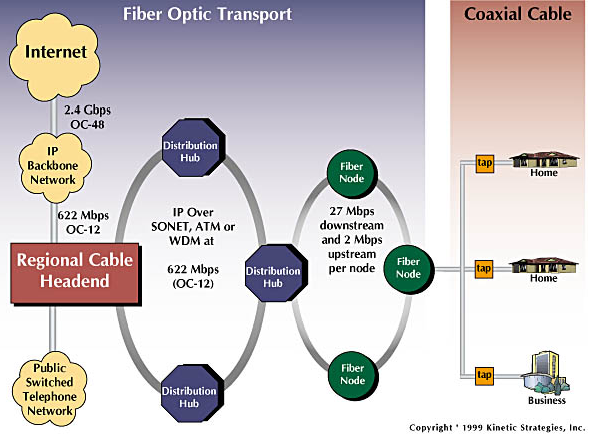
\includegraphics[width=10cm]{imagens/cable.png}
    \label{cable}
    \caption{Cable 1}
\end{figure}
\begin{figure}[h]
    \center
    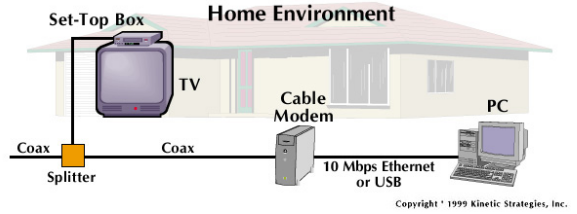
\includegraphics[width=10cm]{imagens/cable2.png}
    \label{cable2}
    \caption{Cable 2}
\end{figure}


\subsection{ADSL}

O ADSL é conhecido pela sua não simetria entre download e upload; O ADSL foi
desenvolvido justamente para isso: Sacrificar o upload em favor do download.\\
A conexão entre o terminal e o modem ADSL ocorre sobre o protocolo Ethernet, mas
entre o modem ADSL e a central da Telecom ocorre sob ATM.
\begin{figure}[h]
    \center
    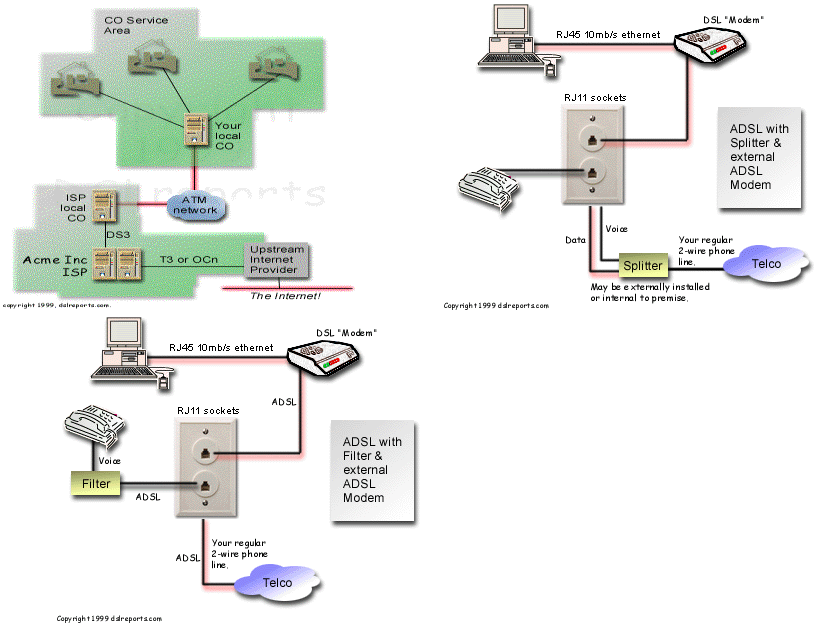
\includegraphics[width=10cm]{imagens/adsl.png}
    \label{adsl}
    \caption{ADSL}
\end{figure}


\subsection{Wireless}

\begin{figure}[h]
    \center
    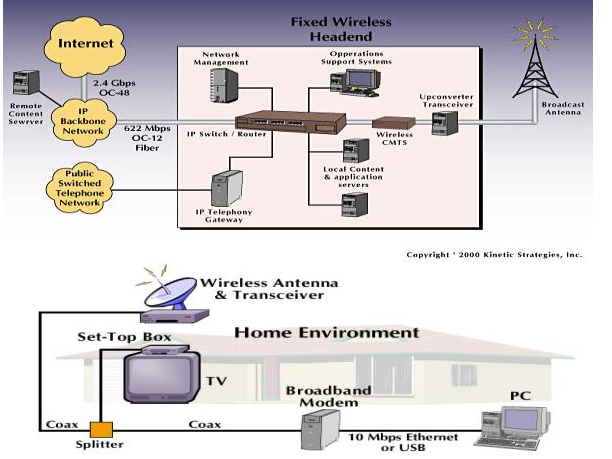
\includegraphics[width=10cm]{imagens/wireless.png}
    \label{wireless}
    \caption{Wireless 1}
\end{figure}
\begin{figure}[h]
    \center
    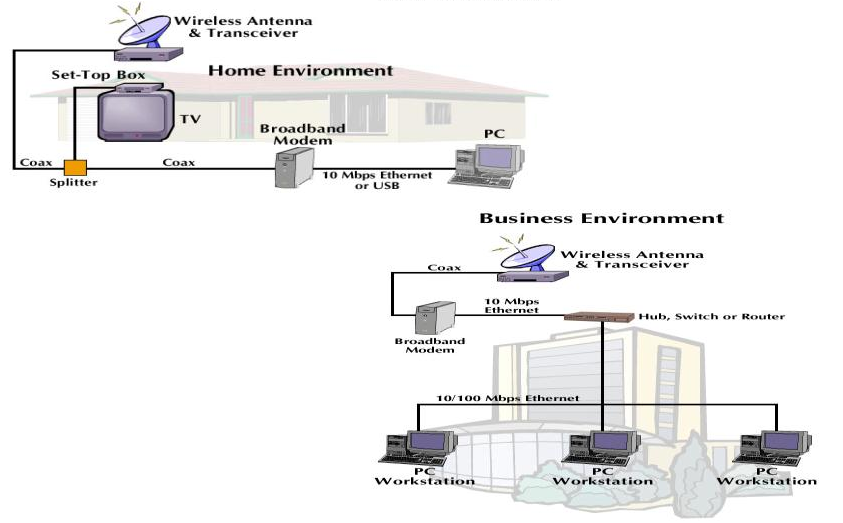
\includegraphics[width=10cm]{imagens/wireless2.png}
    \label{wireless2}
    \caption{Wireless 2}
\end{figure}

\section{Redes sem fio}

\subsection{Padrões}

\begin{itemize}
	\item 802.11: WLAN: Wireless (WiFi)
	\item 802.15: WPAN: Bluetooth
	\item 802.16: WMAN: WiMax
\end{itemize}

\subsection{WiFi}

O modelo WiFi limita a 63 usuários por Access Point; A limitação é feita em
hardware através de um contador que vai de 0 a 63; Como o zero não conta como
conexão, apenas 63 clientes podem se conectar a um AP via
WiFi simultaneamente; Esse limite é apenas uma convenção. \\
Existem dois modelos de redes WiFi:

\begin{itemize}
	\item Com infra-estrutura: \\ Rede com Access Point (AP); Todas as
comunicações passam pelo AP; O AP "manda".
	\item Sem infra-estrutura: \\ Rede sem AP; Máquinas se comunicam
diretamente; É chamada de Rede Ad-Hoc; Máquinas devem servir como routers (rede
multisaltos);
\end{itemize}

\subsection{WiFi: Padrões 802.11}

As siglas (FDM, OFDM etc) serão discutidas mais a frente.

\begin{enumerate}
	\item 802.11a: 5.8ghz, 54mbps no modelo OFDM;
	\item 802.11b: 2.4ghz, 11mbps no modelo FDM;
	\item 802.11g: 2.4ghz, 54mbps no modelo OFDM;
	\item 802.11n: 2.4ghz, 150/300mbps no modelo OFDM
\end{enumerate}

\subsection{Bluetooth}

Esse modelo foi criado para remover fios de periféricos de uma máquina central;
Exemplo: impressora e computador;\\
São 4 as premissas desse modelo: baixo custo, baixo consumo de energia,
pouquíssimo processamento e resistente a interferências.\\
Padrões:
\begin{itemize}
	\item Padrão 1.0: \\ Redes nesse padrão são chamadas de Piconet, formado
por 1 mestre e 7 escravos; Tudo passa pelo mestre e ele manda em todos; Ele
define a hora de falar e a frequência a ser usada.
	\item Padrão 1.1: \\ Chamada de Scatternet, é uma rede que conecta
vários mestes com seus escravos, onde as conexões ocorrem apenas entre mestres,
nunca entre escravos; Eles se conectam de maneira análoga às redes Ad-Hoc; Podem
se conectar no máximo 79 unidades (escravos+mestres).
	\item Padrão 2.0: \\ Foram definidas novas classes e bandas; 100 metros a
1mbps, 10m a 10mbps e, por fim, 1m a 100mbps.
\end{itemize}

A especificação do Bluetooth define três classes de transmissores:

\begin{itemize}
	\item Classe 1:\\ Potência máxima de transmissão de 100 mW, obtendo um
alcance de até 100 metros. 
	\item Classe 2:\\ Potência máxima de transmissão de 2.5 mW, para
alcances de 10 metros.
	\item Classe 3:\\ Potência máxima de transmissão de 1 mW, para alcances
de até 1 metro.
\end{itemize}

A transmissão dos dados é realizada utilizando-se a modulação GFSK \textit{(Gaussian
Frequency Shift Keying)}, sendo o bit 1 representado por uma variação positiva
de frequência e o bit 0 por uma negativa.\\
O acesso ao meio é controlado pelo mestre e é ele quem define a fórmula de salto
de frequência em cada tempo; Para exemplificar: Um mestre define uma fórmula de
saltos para um X tempo, assim ele a cada faixa de tempo trabalhará em uma
frequência diferente, diminuindo assim a probabilidade de sofrer interferência
(ao operar na mesma faixa de frequência que outros aparelhos) e dificulta que o
sinal seja escutado por outro aparelho.\\
Curiosidade: Existem duas maneiras de escutar os sinais de um sinal bluetooth
para roubar os dados trafegados.
\begin{enumerate}
	\item Escutar todas as faixas de frequência e, através de um
algoritmo de força bruta, tentar fazer todas as ligações possíveis dos dados
recolhidos afim de localizar o dado a ser roubado;
	\item Conseguir identificar e roubar a fórmula de frequências enviado pelo mestre ao
seu escravo; Assim você poderá escutar o mestre analogamente ao escravo está
fazendo roubar esses dados. \textit{Don't be cruel}
\end{enumerate}

A imagem abaixo enumera, como exemplo, os saltos de frequência em uma
determinada faixa de tempo; Cores foram usadas para tentar ajudar essa
percepção; Veja os saltos do tráfego de "2": Começa na segunda faixa, depois vai
para a terceira, quarta, primeira, quinta, segunda, terceira e, por fim, quarta
novamente.

\begin{figure}[h]
    \center
    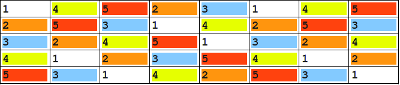
\includegraphics[width=10cm]{imagens/bluetooth.png}
   \label{bluetooth}
    \caption{Bluetooth}
\end{figure}

\section{WiMax}

Padrões:

\begin{itemize}
	\item O padrão 802.16d define conexões de até 72mbps e o uso de antenas
direcionais para um alcance de até 50 milhas;
	\item O padrão 802.16e aumenta as áreas de alcance do WiMax com o uso de
antenas Omnidirecionais, contudo diminui substanciamente seu alcance; 5 milhas
sem LOS (Line-of-sight ou linha de visão, a "visada"); 1,5 milhas sem LOS;
\end{itemize}

Ela pode operar nas faixas entre 3.2ghz, 4,?ghz e 5.8ghz, todas sob OFDM.

\subsection{Frequência vs potência vs qualidade vs alcance}
Quanto maior a frequência (v=lambda*freq), menor será o alcance da antena,
contudo ela trafegará mais dados devido ao tempo ser menor (freq=1/tempo) entre
cada clock. Quanto maior a potência, maior a amplitude do sinal, assim mais
tempo ele levará para virar ruído, aumentando a qualidade e a resistência do
sinal.\\ Trabalhando frequência e potência podemos definir a qualidade de acordo com o
alcance do sinal.

\section{Formas de multiplexação}

Tipos:

\begin{itemize}
	\item TDM (Time Division Multiplexing)
	\item FDM (Frequency Division Multiplexing)
	\item WDM (Wave Division Multiplexing) 
	\item CDM (Code Division Multiplexing) 
\end{itemize}

\subsection{WDM}
Técnica utilizada principalmente em comunicações ópticas, onde os canais
lógicos são caracterizados por um dado comprimento de onda de luz. Através da
técnica de multiplexação por WDM, cada canal TDM ou FDM (que serão explicados
mais adiante), com vários canais associados, pode ser transmitido por uma
determinada cor de luz. Esta luz não está dentro do espectro visível de luz,
mas sim dentro do infravermelho. Então canal de luz comporta-se como uma onda
portadora, com comprimento de luz diferente, podendo transmitir vários canais
TDM ou FDM por comprimento de onda.\\ A multiplexação por WDM não é usada em
redes do tipo LAN, apenas em sistema de telefonia, CATV e telecomunicações
intercontinentais. Nestes sistemas, as taxas de transmissão necessitam de
sistemas ópticos complexos, que tornam-se  economicamente inviáveis para as
redes locais LAN's.

\begin{figure}[h]
    \center
    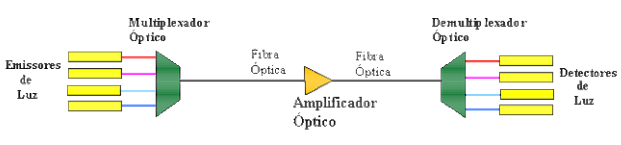
\includegraphics[width=10cm]{imagens/wdm.png}
    \label{wdm}
    \caption{WDM}
\end{figure}

\subsection{CDM}
Os sinais são separados por técnicas de codificação, mas misturados em
tempo e freqüência. Todos os sinais podem ser transmitidos simultaneamente, com
a mesma freqüência da portadora. 

\subsection{FDM}
Cada canal de informação é associado a uma Portadora específica, com freqüência,
fase ou amplitude diferentes, sendo depois multiplexados em um único canal de
transmissão através de uma matriz de  resistores, sendo depois amplificado. O
sinal resultante é um sinal composto por vários sinais com portadoras discretas,
também chamadas de canais intermediários, que são separadas no receptor por
filtros e demoduladores, cada um sintonizado em uma freqüência de portadora
especifica.

\subsection{TDM} É um sistema de multiplexação onde cada canal de informação é
associado à um intervalo de tempo; Para que se possa fazer esta associação, cada
canal de informação colocado em um BUFFER de memória. A eficiência de modo de
transmissão digital multiplexada por TDM é muito maior que a FDM, pois requer um
menor número de repetidores, cerca de um a cada 30 ou 40km, mas uma das
desvantagens dos sistemas TDM é que temos que acrescentar ao sinal original uma
quantidade de BITs de informação; Esses BITs são para o sincronismo de
multiplexação e desmultiplexação, detecção de erro e para o gerenciamento da
rede.

\begin{figure}[h]
    \center
    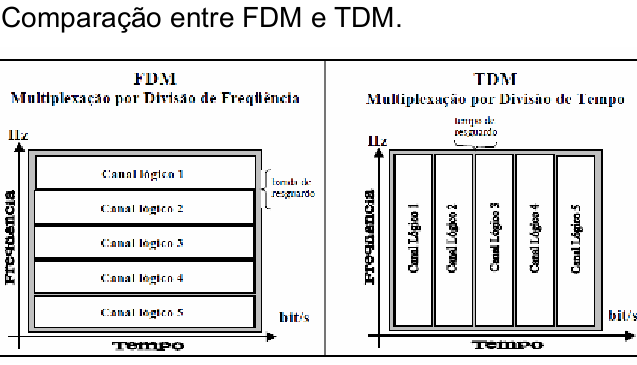
\includegraphics[width=10cm]{imagens/fdmtdm.png}
    \label{fdmtdm}
    \caption{FDM e TDM}
\end{figure}

\subsection{Curiosidade: O OFDM}
Usado pelo ADSL e também por alguns dos padrões 802.11 e na Hyperlan (padrão
WiFi europeu), merece uma introdução nessa apostila; Devido a sua complexidade,
ele não será muito estudado. \\ O OFDM \textit{(Orthogonal frequency-division
multiplexing)} também conhecido como DMT \textit{(Discrete Multitone
Modulation)}, é uma técnica de modulação baseada na idéia de multiplexação por
divisão de frequência (FDM) onde múltiplos sinais são enviados em diferentes
frequências.\\ Muitos são familiarizados com FDM pelo uso de aparelhos de rádio
e televisão: Normalmente, cada estação é associada a uma determinada frequência
(ou canal) e deve utilizá-la para realizar suas transmissões.\\ O OFDM parte
deste conceito e vai além, pois divide uma única transmissão em múltiplos sinais
com menor ocupação espectral (dezenas ou milhares); Isso adicionado com o uso de
técnicas avançadas de modulação em cada componente, resulta em um sinal com
grande resistência à interferência.\\ O OFDM é quase sempre utilizado juntamente
com codificação de canal (técnica de correção de erro), resultando no chamado
COFDM.

\begin{figure}[h]
    \center
    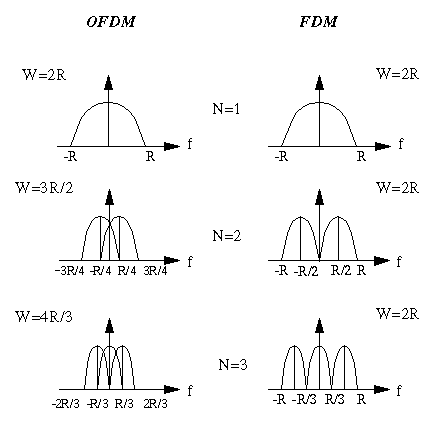
\includegraphics[width=10cm]{imagens/ofdm.png}
    \label{ofdm}
    \caption{OFDM}
\end{figure}

\section{Codificação de sinal}

Tipos:

\begin{itemize}
	\item NRZ-L, Non-return to Zero Level
	\item AMI, Alternated Mark Inversion
	\item Manchester, usado no protocolo Ethernet
	\item Manchester diferencial
\end{itemize}

\subsection{Manchester} Neste esquema os pulsos elétricos enviados só têm
significado aos pares: a cada par de pulsos enviados, se o primeiro for mais
forte que o segundo, indica a transmissão de um 1. Inversamente, se o primeiro
for mais fraco que o segundo, indica a transmissão de um 0. Assim, quando não
houver transmissão, todos os pulsos serão fracos ou simplesmente inexistentes.\\
Para exemplificar, imagine a seguinte seqüência de pares de pulsos enviados:
(alto baixo), (alto baixo), (alto baixo), (baixo alto), (alto baixo). Nesta
codificação os números transmitidos seriam 11101.\\ A sua principal vantagem é a
facilidade de se recuperar erros. Mesmo que parte da transmissão se perca, ainda
assim é fácil detectar qual foi o sinal enviado; Uma desvantagem da codificação
Manchester é que ela exige duas vezes mais largura de banda que a codificação
binária direta, pois os pulsos são a metade da largura. Por exemplo, para
transmitir dados a 10 Mbps, o sinal tem de mudar 20 milhões de vezes por
segundo.

\begin{figure}[h]
    \center
    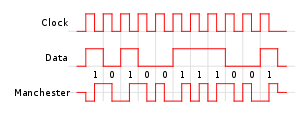
\includegraphics[width=10cm]{imagens/manchester.png}
    \label{manchester}
    \caption{Manchester}
\end{figure}

\subsection{Manchester diferencial}
Os bits também são representados por pares de pulsos, só que, se o primeiro
pulso de um par for da mesma intensidade do segundo pulso do par anterior, ou
seja, não houve uma transição, há a transmissão de um 1; Já se o primeiro pulso
de um par for de intensidade diferente do segundo pulso do par anterior, ou
seja, houve uma transição, há a transmissão de um 0.
\begin{figure}[h]
    \center
    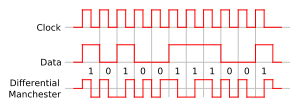
\includegraphics[width=10cm]{imagens/manchesterdiff.png}
    \label{manchesterdiff}
    \caption{Manchester diferencial}
\end{figure}

\subsection{NRZ-L}
É a codificação mais simples. Representamos o 1 por um sinal negativo e o 0 por um sinal positivo. Problema grave: Se tivermos de enviar muitos sinais repetidos (como, por
exemplo, um monte de 1), corremos o risco de perder a sincronia dos dados.\\
Importante: Eu errei isso em prova porque vários sites ensinam errado (wikipedia, sites da ufsc, ufce etc): Não existe codificação NRZ. NRZ é uma categoria que se divide em NRZ-Inverse (NRZ-I) e NRZ-Level (NRZ-L). O NRZ-L é o explicado acima. O NRZ-I não foi ensinado no meu semestre e funciona num esquema diferente.


\subsection{AMI}
A representação do 1 será feita com uma voltagem negativa ou positiva e o 0 será
representado por 0 volts.

\begin{figure}[h]
    \center
    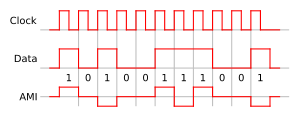
\includegraphics[width=10cm]{imagens/ami.png}
    \label{ami}
    \caption{AMI}
\end{figure}


\subsection{NRZ vs Manchester}

Tabela comparativa bem interessante.

\begin{figure}[h]
    \center
    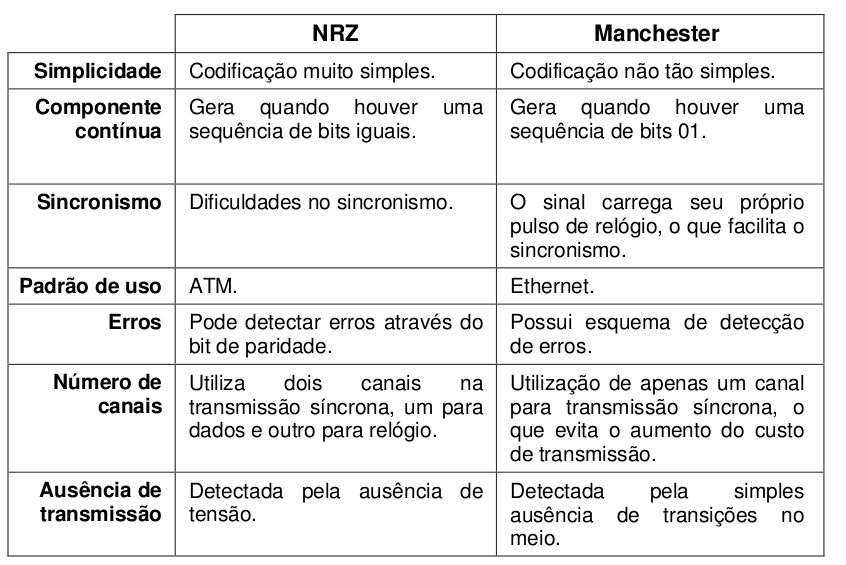
\includegraphics[width=10cm]{imagens/nrzmanchester.png}
    \label{nrzmanchester}
    \caption{NRZ vs Manchester}
\end{figure}

\section{Topologias de Rede}

Existem diversas topologias de rede, cada qual tendo suas vantagens e
desvantagens em relação à eficiência, taxa de entrega, tráfego de dados, número
de colisões, custo etc.

\begin{figure}[h]
    \center
    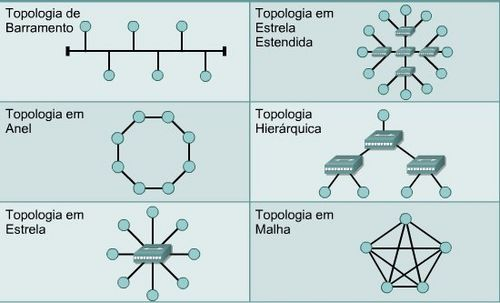
\includegraphics[width=10cm]{imagens/topologias.jpg}
    \label{topologias}
    \caption{Topologias}
\end{figure}

\subsection{Barramento}
Todas as máquinas usam a mesma rede; Apenas uma transmite por vez; Baixíssimo
custo; Muito ineficiente: alto número de colisões e baixo tráfego de dados por
segundo.

\subsection{Ponto a Ponto}
São redes em que dois equipamentos ligam-se direramente sobre algum protocolo, como
o PPPoE (Point to Point Protocol over Ethernet) e o PPPoA (Point to Point
Protocol over ATM).\\
Exemplo comum de uso em casa: Rede até um modem ADSL opera sobre PPPoE, e do
modem ADSL para a Telecom opera-se sobre PPPoA.

\subsection{Hierárquica ou Árvore}
Topologia com hierarquia com várias ramificações conectadas em nodos em comum;
Muito utilizada para supervisionar aplicações de tempo real, como por exemplo
transações bancárias (já viu um terminal eletrônico bancário exibir a mensagem "Autenticando a transação na central(...)"?

\subsection{Estrela}
Os pontos se conectam a um nó em comum, o concentrador; A vantagem do
concentrador é permitir mais tráfego de diferentes máquinas ao mesmo tempo; Mas
cuidado: Se usado com um HUB, você obtém um barramento; Se usado com um Switch,
você está com uma topologia em estrela.

\subsection{Estrela estendida}
Expansão do formato estrela; A figura acima (figura 15) torna a ideia mais clara.

\subsection{Anel}
Pode ser compreendida como uma rede de barramento sem começo ou fim; Apenas uma
máquina fala por vez. É igualmente ruim como o barramento, contudo, través de um
sistema de prioridades, pode ser usada para trafegar uma enorme quantidade de
dados; Exemplos: Topologias Token Ring e FDDI.

\subsection{Malha}
Todos os nós estão interligados uns aos outros; Reduz drasticamente o número de
colisões, mas torna a rede complexa, aumenta o gasto com cabeamento e com placas de
rede; Topologias em malha são muito usadas em clusters, como por exemplo: Torus,
Hipercubo e em Árvore.

\subsection{Híbrida}
Quando você mistura duas redes. Imagine duas estrelas ligadas por um
barramento.

\begin{figure}[h]
    \center
    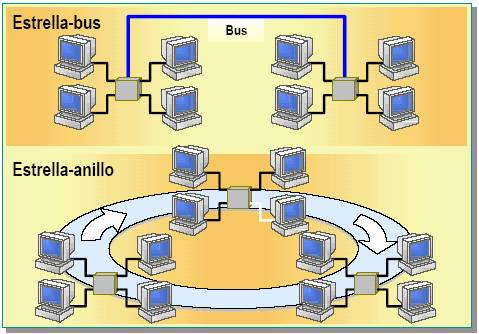
\includegraphics[width=10cm]{imagens/hibridas.jpg}
    \label{hibridas}
    \caption{Híbridas}
\end{figure}

\subsection{Regra 5-4-3}
Uma rede ethernet a 10mbps pode ter no máximo 5 segmentos conectados por no
máximo 4 repetidores, sendo que no máximo 3 desses segmentos podem estar
povoados (com máquinas transmitindo); A regra 5-4-3 é uma convenção para redes
de 10mbps, pois acima dessas restrições a rede passa a ter taxas inferiores a
20\% de entrega, tornando-a extremamente ineficiente. O comprimento máximo dessa
rede será de 925metros.\\
Tente identificar essa regra na imagem abaixo. Identifique os segmentos povados
e não povoados. Podem parecer difícil, mas com calma você compreenderá e não
mais esquecerá.

\begin{figure}[h]
    \center
    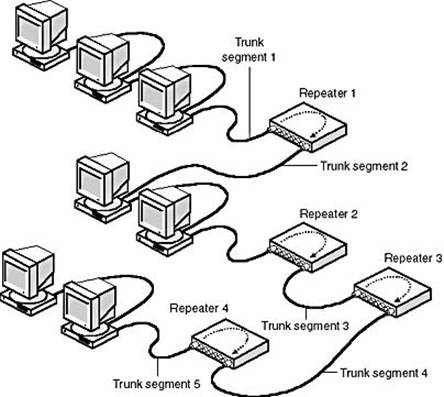
\includegraphics[width=10cm]{imagens/543.png}
    \label{543}
    \caption{Regra 5-4-3}
\end{figure}


\section{Token Ring}
Se você tem uma grande quantidade de pessoas querendo falar (numa reunião por
exemplo), como fazer para que apenas uma fale de cada vez? Uma solução seria
usar um bastão de falar: quem estivesse com o bastão (e somente ele) poderia
falar por um tempo determinado, ao final do qual deveria passar o bastão para
outro que quisesse falar e esperar até que o bastão volte, caso queira falar
mais.\\ É justamente este o sistema usado em redes Token Ring. Um pacote especial,
chamado pacote de Token circula pela rede, sendo transmitido de estação para
estação. Quando uma estação precisa transmitir dados, ela espera até que o
pacote de Token chegue e, em seguida, começa a transmitir seus dados.\\ A transmissão de dados em redes Token também é diferente. Ao invés de serem
irradiados para toda a rede, os pacotes são transmitidos de estação para estação
(daí a topologia lógica de anel). A primeira estação transmite para a segunda,
que transmite para a terceira, etc. Quando os dados chegam à estação de destino,
ela faz uma cópia dos dados para sí, porém, continua a transmissão dos dados. A
estação emissora continuará enviando pacotes, até que o primeiro pacote enviado
dê uma volta completa no anel lógico e volte para ela. Quando isto acontece, a
estação pára de transmitir e envia o pacote de Token, voltando a transmitir
apenas quando receber novamente o Token.\\ O sistema de Token é mais eficiente em redes grandes e congestionadas, onde a
diminuição do número de colisões resulta em um maior desempenho em comparação
com redes Ethernet semelhantes. Porém, em redes pequenas e médias, o sistema de
Token é bem menos eficiente do que o sistema de barramento lógico das redes
Ethernet, pois as estações têm de esperar bem mais tempo antes de poder
transmitir.

\subsection{FDDI}

As redes FDDI adotam uma tecnologia de transmissão idêntica às das redes Token
Ring, mas utilizando, vulgarmente, cabos de fibra óptica, o que lhes concede
capacidades de transmissão muito elevadas (em escala até de Gigabits por
segundo) e a oportunidade de se alargarem a distâncias de até 200 Km, conectando
até 1000 estações de trabalho. Estas particularidades tornam esse padrão
bastante indicado para a interligação de redes através de um backbone, nesse
caso, o backbone deste tipo de redes é justamente o cabo de fibra óptica duplo,
com configuração em anel FDDI, ao qual se ligam as sub-redes. FDDI utiliza uma
arquitetura em anel duplo. \\Atenção: O FDDI é uma Toekn Ring com o uso de fibra óptica e com
prioridade

\section{Colisões de Rede}

Falarei aqui sobre as colisões de dados na rede; Recomendo fazer uma leitura
sobre a história da rede Aloha, pois é assunto em classe e de prova; Dissertarei
especificamente sobre o que interessa para a prova.

\subsection{Aloha Puro}
O transmissor envia o dado sem qualquer regra; Ele fica escutando a rede; Se o
seu pacote foi destruído, ele espera um tempo aleatório e envia novamente, sem
qualquer regra. Se não for possível escutar a rede, serão necessárias
confirmações (ACK ou NACK).

\subsection{Aloha Discreto}
Divide o tempo em intervalos discretos, e cada intervalo corresponderá a um
quadro e passa a exigir que os transmissores concordem em relação às fronteiras
dos slots. Para alcançar essa concordância, poderíamos, por exemplo, ter uma
estação que enviasse um sinal sonoro no início de cada intervalo. Em outras
palavras, só se transmite agora no início do próximo slot.

\subsection{CSMA/CD}
O CSMA/CD \textit{Carrier Sense Multiple Access with Collision Detection} é
caracterizado por todos os nós enquanto transmitem, também escutem (L.W.T. ou
Listen While Talk). Quando ele detecta uma colisão na rede, ele emite um sinal
chamado JAM, de 48 bytes, para anunciar que ocorreu uma colisão. Para evitar uma
nova colisão, ele espera um tempo aleatório e tenta transmitir novamente.\\
O CSMA/CD garante 95\% de taxa de entrega; O menor pacote no CSMA/CD é de 64
bytes; Embora pareça uma informação superficial, é muito importante pois já foi
uma questão de diversas provas. Esse sistema de colisão, usado no modelo
Ethernet, exige que o menor pacote válido seja de 64 bytes; O maior pacote será
de 1518 bytes, mas essa não é uma informação importante.\\
Mas por qual motivo 64 bytes? Em redes até 100mbps, 64bytes é a quantia de bytes
necessária para tentar garantir que quando o byte número 63 (último byte) estiver sendo
transmitido, o primeiro byte já tenha chegado, ocupando todo o "cabo" ou "túnel"
entre a origem e o destino; Para redes fast ethernet (como a de 100mbps) foi
necessário aumentar o tamanho do pacote mínimo (512bytes).

Passo-a-passo:

\begin{enumerate} 
	\item Se o canal está livre, inicia-se a transmissão, caso contrário vai para o passo 5;
	\item (transmissão da informação): Se uma colisão é detectada, a
transmissão continua até que o tempo mínimo para o pacote seja alcançado (para
garantir que todos os outros transmissores e receptores detectem a colisão),
então segue para o passo 5; 
	\item (fim de transmissão com sucesso): Informa sucesso para as camadas de rede superiores, sai do modo de transmissão;
	\item (canal está ocupado): Espera até que o canal esteja livre;
	\item (canal se torna livre): Espera-se um tempo aleatório, e vai para o passo 2, a  menos que o número máximo de tentativa de transmissão tenha sido excedido;
	\item (número máximo de tentativa de transmissão excedido): Informa
falha para as camadas de rede superiores e sai do modo de transmissão;

\end{enumerate}

\subsection{CSMA/CA}
O CSMA/CA \textit{Carrier Sense Multiple Access with Collision Avoidance} é bem
mais ordenado que o CSMA/CD, o que contribui fortemente para a diminuição do
número de colisões, chegando a uma taxa de entrega de até 99\% dos dados.\\
Antes de transmitir um pacote, uma estação envia um RTS (Request to Send)
avisando que vai transmitir e quanto tempo vai demorar para concluir; Dessa
maneira, a outra estação irá ficar escutando. Vou tentar explicar com um
exemplo para facilitar a compreensão:\\
A estação A envia um RTS-B (com quem quer falar); Obviamente todos no alcance de
A receberão esse RTS; Todos ficarão em silêncio, inclusive B, mas B enviará um
CTS-A (Clear to Send para A), e todos do alcance de B ficarão em silêncio.\\
Esse modelo é normalmente usado em redes Wireless (WiFi), mas pode ser usado em
uma rede cabeada; Esse sistema de detecção de colisão consegue garantir 100\% de
taxa de entrega na rede cabeada, mas torna-a também muito mais lenta.

\subsection{1-p-CSMA, p-CSMA e np-CSMA}
Na np-CSMA \textit{(non-persistent CSMA)}, quando a transmissora percebe que o
meio está ocupado, ela espera um tempo aleatório para tentar novamente
transmitir seus dados.\\ Já a p-CSMA \textit{(persistent CSMA)} transmite seus
dados com uma probabilidade X de acertar ou espera um tempo aleatório e tenta
transmitir com uma probabilidade X de acertar; Segue assim até conseguir
transmitir ou até que uma outra estação ganhe acesso ao canal. \\ A 1-p-CSMA é a
mesma coisa que a p-CSMA com uma única subtração: Espera o meio ficar livre para
transmitir (embora isso possa demorar e resultar em colisões da mesma maneira).

\section{ARP}
O ARP \textit{Address Resolution Protocol} é atualmente usado para encontrar um
endereço da camada de Enlace (como na Ethernet) a pártir de um endereço da
camada de rede (como um endereço IP); Em outras palavras, na prática, ele traduz
um endereço IP para um endereço MAC.

\section{RARP}
Faz o contrário do ARP, isto é, transforma um endereço MAC em um endereço IP.

\section{Cabos}

É uma parte extensa da matéria e envolve muitos números. Normalmente não é
cobrado que o aluno decore todos os cabos, mas tenha uma notação dos principais
tipos e modelos usados. Obviamente, portanto, falarei apenas dos mais
importantes.

\subsection{Fibras ópticas}
Desvantagens:
\begin{itemize}

	\item Custo ainda elevado de compra e manutenção;
	\item Fragilidade das fibras ópticas sem encapsulamento;
	\item Dificuldade de conexões das fibras ópticas;
	\item Acopladores tipo T com perdas muito grandes;
	\item Impossibilidade de alimentação remota de repetidores;
	\item Falta de padronização dos componentes ópticos.
\end{itemize}

\subsection{Fibras Monomodo}
\begin{itemize}
	\item Permite o uso de apenas um sinal de luz pela fibra;
	\item Dimensões menores que os outros tipos de fibras;
	\item Maior banda passante por ter menor dispersão;
	\item Geralmente é usado laser como fonte de geração de sinal;
\end{itemize}

\subsection{Fibras Multimodo}
\begin{itemize}
	\item Permite o uso de fontes luminosas de baixa ocorrência tais
como LEDs (mais baratas);
	\item Diâmetros grandes facilitam o acoplamento de fontes
luminosas e requerem pouca precisão nos conectores;
	\item Muito usado para curtas distâncias pelo preço e facilidade
de implementação pois a longa distância tem muita perda.
\end{itemize}

\subsection{Cat 5, 5e, 6 e 6a}
O cabo Cat5 é requisito mínimo para operar em redes de 10, 100 e 1000mbps,
suportanto frequências de até 100mhz.\\ A versão Cat 5e ("e" de "enhanced") visa
aperfeiçoar o cabo Cat5 ajudando a diminuir a interferência e perda do sinal, o
que se traduz em cabos mais longos, até 100metros; Esses cabos operam também em
100mhz, mas agora essa especificação é mínima e pode-se ter cabos Cat 5e
suportando frequências superiores.\\ Cabo Cat 6 suportam frequências de até 250mhz e foram
feitos para redes 10gbps em até 55metros; Para expandir para 100metros, foi
criado o Cat 6a ("a" de "augmented"), suportando frequências de até 500mhz. A
espessura desse tipo de cabo aumentou devido a criação de um separador de cabos
para reduzir a interferência entre os pares de cabos).

\section{O modelo Ethernet} 
A raínha das questões de prova merce uma atenção especial em todos os aspectos
discutidos em classe.\\
A Ethernet é uma tecnologia de interconexão para redes locais (LAN) baseada no
envio de pacotes; Ela define um conjunto de características, como cabeamento e
sinais elétricos para a cadama Física e o formato dos pacotes e protocolos para
a camada de acesso ao meio (MAC, Media Access Control) de acordo com o modelo da
OSI discutido no início dessa apostila.\\
A Ethernet foi padronizada pela IEE como 802.3. É a tecnologia de LAN mais usada
no mundo e tem tomado grande espaço de algumas redes como a Token RIng, FDDI e
ARCNET.\\
Cada ponto possui uma chave de 48 bits globalmente única chamada endereço MAC,
assegurando que pelo menos teoricamente todos os sistemas ethernet tenham
endereços distintos.\\

Pontos importantes:

\begin{itemize}
	\item Tamanho mínimo de um pacote: 64bytes para ethernet e 512bytes para
fast ethernet; A razão já foi discutida na explicação do modelo CSMA/CD;
	\item Codificação usada: Manchester
	\item Sistema de comunicação usado: CSMA/CD;
	\item Modelo ethernet tem tamanho de pacote máximo de 1518bytes;
	\item Sistema de controle de fluxo: Janelas Deslizantes
	\item Endereço MAC: 48 bytes, 12 dígitos em hexa. Os 3 primeiros
identificam a fabricante e os 3 seguintes são identificações fornecidas pela
fabricante; 
	\item Sistema de detecção de erros: CRC-32 implementada em hardware;
\end{itemize}

\subsection{MAC}
A IEEE define três categorias gerais de endereços MAC em Ethernets:

\subsection{Endereços Unicast}
Um endereço MAC que identifica uma única placa de interface LAN.

\subsection{Endereços Broadcast}
O tipo de MAC do grupo IEEE mais utilizado, tem um valor de FFFF.FFFF.FFFF (em notação hexadecimal). O endereço broadcast implica que todos os dispositivos na LAN devem receber e processar um quadro enviado ao endereço broadcast.

\subsection{Endereço Multicast} Quadros enviados para unicast são destinados a um único dispositivo; quadros enviados para um endereço broadcast, são destinados à todos os dispositivos. Os quadros enviados a endereços multicast, são destinados a todos os dispositivos que se interessem em receber o quadro.

\section{Virtual LAN}
Uma rede local virtual, normalmente denominada de VLAN, é uma rede logicamente
independente. Várias VLAN's podem co-existir em um mesmo comutador (Switch). O
protocolo predominante é o IEEE 802.1Q. As primeiras VLAN's geralmente eram
configuradas para reduzir o tamanho do domínio de colisão em um segmento
Ethernet muito extenso para melhorar o desempenho. Quando os Switch's
diminuíram esse problema (diminuíram porque eles não têm um domínio de colisão), as
atenções se voltaram para a redução do domínio de broadcast na camada MAC.
Dependendo do tipo de configuração, os usuários ganham mobilidade física dentro
da rede.\\ Um outro propósito de uma rede virtual é restringir acesso a recursos
de rede sem considerar a topologia da rede, porém este método é questionável.

\section{Janelas Deslizantes}
Assunto recorrente em aula, trabalhos e provas, de grande importância. Depois do modelo Ethernet, é o tema mais discutido. As Janelas deslizantes controlam o fluxo dados dados e é usado no modelo Ethernet, conforme já foi dado a devida ênfase.\\ Explicarei aqui as Janelas deslizantes Volta-N, contudo existe o modelo de Janelas Deslizantes com buffer, normalmente não abordado em classe, mas passível de ser.\\ IMPORTANTE: O tamanho da janela SEMPRE será configurado pelo RECEPTOR. O TRANSMISSOR pode encher essa janela ou não, mas NUNCA enviar mais que o tamanho da janela configurado pelo RECEPTOR!

\subsection{Janelas Deslizantes Volta-N}
Modelo normalmente discutido em classe, é simples e fácil de ser entendido.\\
Imagine que você tem que enviar uma sequência de 3 bits de pacotes, portanto uma sequência de 0 a 7. Imagine que os números ímpares sempre retornem um NACK na primeira vez que são enviados, isto é, não sejam entregues na primeira tentativa; Imagine ainda uma janela de tamanho 3.\\
\begin{enumerate}
	\item Tentamos enviar os pacotes 0, 1 e 2.
	\item O 1 recebe NACK. A janela volta para o primeiro que falhou; A janela deslizante agora será 1, 2 e 3;
	\item O 3 recebe um NACK; A nova janela será 3, 4 e 5.
	\item O 5 recebe um NACK; A nova janela será 5, 6 e 7.
	\item o 7 recebe um NACK; A nova janela será 7.
	\item Observe: A janela volta para o primeiro erro da sequência e reenvia TUDO de novo;
\end{enumerate}

\section{Celulares}

A história sobre as gerações de tecnologias em rede celulares é longa, embora
interessante. Irei me ater a questões de provas.

\subsection{1G}
Uso de padrões analógicos de transmissão e recepção.\\
Problemas: Distorção de voz e instabilidade na rede.

\subsection{2G}
Uso de padrões digitais de transmissão e recepção.\\
Início da possibilidade de troca de dados, como envio de torpedos, e a introdução
de multiplexação dos dados, permitindo que várias informações trafegassem sem
que uma intereferrise na outra.\\
Padrões usados: TDMA, CDMA e GSM; O GSM é baseado no TDMA; O GSM teve sucesso
devido ao seu uso em larga escala por várias operadoras; O CDMA melhorou o
sistema de multiplexação de dados.

\subsection{2,5G}
Primeiro deve ficar claro que o 2,5G não existe oficialmente segundo a União
Internacional de Telecomunicações (UIT). Ela define a transição de tecnologia 2G
para 3G. A inclusão da rede EDGE (para GSM) e 1xRTT (para CDMA) para transmissão
mais rápida de dados. O EDGE é um GPRS com mais banda, também conhecido como
enhanced-GPRS ou somente e-GPRS.\\
Problema: Capacidade de transmissão de dados muito limitada.

\subsection{3G}
Maior capacidade de transmissão de dados em relação ao 2G; Suporta um número
maior de clientes de voz e dados;

\subsection{4G}
Ainda sob definição, irá introduzir com sustentabilidade recursos como MMS
(Multimedia Messaging Service), Video Chat, mobile TV, conteúdo HDTV, DVB
(Digital Video Broadcasting) etc com banda mínima de 100mbps para máquinas
móveis e 1gbps para fixas e interoperabilidade entre diversos padrões de rede
sem fio.

\section{Detecção de erros}
Métodos de detecção de erros.

\subsection{CRC}
Existem vários CRC, mas o bom é lembrar que o método usado na ethernet é o CRC-32; Bom também lembrar que ele é rápido porque ele foi pensado para ser implementado em hardware.

\subsection{Paridade ímpar: Vertical, Horizontal e Longitudinal}
Vou direto para um exemplo.

\begin{enumerate}
	\item Vamos transmitir a seguinte mensagem de 40 bits:\\
		1110101110001010111000010101110100001101
	\item Primeiro separamos em blocos de 8 bits por linha (motivo: 8 bits = 1 byte):\\
		11101011\\
		10001010\\
		11100001\\
		01011101\\
		00001101\\
	\item Para verificar a paridade horizontal ímpar, contamos o número de "1" por linha; Se der ímpar, o bit de paridade será 0. Se par, 1. Na verdade ocorre um XOR dos bits. Veja:\\
                11101011 - 1\\
                10001010 - 0\\
                11100001 - 1\\
                01011101 - 0\\
                00001101 - 0
	\item Para verificar a paridade vertical ímpar, fazemos a mesma coisa, mas com as colunas:\\
                11101011\\
                10001010\\
                11100001\\
                01011101\\
                00001101\\
		00101101 - paridade vertical
	\item A paridade longitudinal significa que devemos fazer a mesma coisa agora com os bits de paridade vertical e horizontal. Se os bits de paridade baterem, a paridade longitudinal é verificada. Veja:\\
		Horizontal:	00101100, bit de paridade: 0\\
		Vertical:	01011, bit de paridade: 0\\
		Longitudinal: 0\\
		Longitudinal: if (horizontal==vertical) \{longitudinal bateu! \} else \{nao bateu\} 
\end{enumerate}

\subsection{Paridade par}
Exatamente a mesma idéia acima, mas quando você tiver um número ímpar de "1", o bit de paridade será 1. Se der par, será 0.


\section{Questões de prova}
Cada subseção será uma pergunta e o seu conteúdo a resposta; A maioria das
questões vieram de provas; Pouquíssimas questões foram criadas por focarem
pontos importantes da matéria.

\subsection{Diferencie cabo par trançado categoria 5, 5e e 6, fibra óptica e cabo coaxial. Cite
seus principais usos. Diferencie roteador e switch. Mostre três exemplos de
topologia de rede em desenhos (1,0)}
O cabo cat5 opera em até 100mhz e é capaz de transmitir 10/100/1000. Cabo 5e tem no
mínimo 100mhz de frequência para suportar e aumenta a transmissão de 1000mbps
para 100metros. Cabo cat6 opera em até 250mhz e permite 10gbps até 55 metros.
Cabo cat 6a expande esse limite para 100 metros, implementa separador de pares
de cabo para diminuir a interferência e, por fim, permite operar em frequências
até 500mhz.

\subsection{Explique o funcionamento do CSMA/CD e do CSMA/CA. Por que o quadro mínimo do
CSMA/CD é de 64 bytes? (1,0)}
CSMA/CD: Listen While Talk. CSMA/CA: Request to Send e Clear to Send. 64bytes é
o pacote mínimo do CSMA/CD; Leia mais informações nas respectivas seções. É importante também citar como o CSMA/CD percebe uma colisão (variação de amplitude do sinal) e o tamanho do pacote mínimo. Não comentar isso pode reduzir a sua nota.

\subsection{Demonstre o funcionamento do protocolo janelas deslizantes para comunicação
entre duas máquinas usando volta-N. Devem ser transmitidas 20 mensagens, sendo
que o número de sequência delas é representado por 4 bits. O tamanho inicial da
janela é de 3 mensagens e deve ser alterado para 5 logo após a 12a mensagem e
para 2 após a 16a mensagem. As mensagens com número de sequência ímpar são
sempre transmitidas com erro da primeira vez e corretamente na segunda. A 14a
mensagem deve ser retransmitida 4 vezes até chegar completamente. (2,0)}

\begin{enumerate}
	\item Mensagens: 0-1-2-3-4-5-6-7-8-9-10-11*-12-13*-14-15*-0-1-2-3
	\item |0|1|2|
	\item |1|2|3|
	\item |3|4|5|
	\item |5|6|7|
	\item |7|8|9|
	\item |9|10|11|
	\item |11|12|13|
	\item |13|14|15|0|1|
	\item |13|14|15|0|1|
	\item |13|14|15|0|1|
	\item |13|14|15|0|1|
	\item |15|0|1|2|3|
	\item |1|2|
	\item |3|
\end{enumerate}

\subsection{Explique como funciona a duplexação por divisão de tempo e por divisão de
frequência. Como ela pode ser usada em conjunto com as técnicas de acesso
múltiplo por divisão de tempo, por divisão de frequência e por divisão de
código. (1,0)}

\subsection{Escolha um endereco IP classe B. Divida essa rede em 12 subredes. Mostre
quais são os endereços de rede de cada uma das subredes, mostre qual é o
endereço de broadcast de cada uma das subredes, mostre qual a máscara utilizada
por cada uma das subredes. (2,0)}

\subsection{Explique o funcionamento de  três esquemas de condificação digital de dados,
é obrigatório que um deles seja o código manchester. (1,0)}
Explicado em seções anteriroes.

\subsection{Ethernet (1,0). A - Como é o endereçamento das placas ethernet? Como ele é dividido e o que
representa cada parte?}
Chamados de MAC ADDRESS; Possui 48bits ou 12 dígitos em hexa. Os 3 primeiros
dígitos hexa informam a fabricante e os 3 seguintes informações do fabricante.

\subsection{Ethernet (cont.). B - Qual a técnica de controle de fluxo, de detecção de erros e de codificação
usada pela ethernet?}
Janelas Deslizantes. CRC-32. Manchester.

\subsection{Ethernet (cont.). C - Qual é o tamanho mínimo das mensagens ethernet? Porque elas tem esse valor?}
64 bytes. Explicado no capítulo sobre CSMA/CD.

\subsection{Diferencie ADSL e Cable Modem (1,0)}
A conexão entre o modem ADSL e o terminal ocorre sob Ethernet. A conexão entre o modem ADSL e o ISP (Internet Service Provider) ocorre sobre protocolo ATM e em cabo de cobre. Uma característica importante do ADSL é a taxa de upload ser reduzida para permitir mais download.\\
A conexão entre o modem CABLE e o terminal ocorre sob Ethernet. A conexão entre o modelo CABLE até o ISP primeiro passa pelos Fiber Node e Hubs de distribuição. Do ISP até os hubs de distribuição ocorre sob fibra e SONET/ATM/WDM. Dos Fiber Node até o modem Cable ocorre sob cabo coaxial. É possível implementar tudo sobre fibra.

\subsection{Explique o funcionamento das modulações de amplitude, frequência e fase. (1,0)}
Modulação é o processo onde é alterada alguma característica de um sinal
(chamado de portadora) em função de outro (chamado de sinal modulante que contém
a informação).

\begin{itemize}
	\item Modulação em amplitude (AM). Opera na faixa dos Khz, com ondas de
baixa frequência. Garante um longo alcance, porém são mais suscetíveis a ruídos.
Frequência e fase são mantidas constantes. Obviamente a amplitude é modificada.
	\item Modulação em frequência (FM). Opera na faixa dos Mhz, com
qualidade maior por permitir mais dados devido as frequências altas, mas pelo
mesmo motivo diminui o seu alcance. Amplitude constante, mas fase varia.
	\item Modulação em fase (PM). Vários desvios nas fases ocorrem.
Amplitude constante, mas frequência varia.
\end{itemize}

\subsection{Explique o funcionamento dos protocolos ARP, RARP, para que eles servem? (0,5)}
ARP traduz IP para MAC; RARP traduz um MAC para IP.

\subsection{Diferencie em uma tabela celulares de 1G/2G/2,5G/3G (0,5)}
1G opera sobre padrões analógicos. 2G introduz padrões digitais e transmissão de
dados. 2,5G não é oficial e caracteriza a transição de 2G para 3G. 3G introduz
maiores capacidades de banda e maior número de clientes de voz e dados.

\subsection {Diferencie 802.11 a/b/g/n (1,0)}
\begin{itemize}
	\item 802.11a: 5.8ghz, 54mbps, OFDM
	\item 802.11b: 2.4ghz, 11mbps, FDM
	\item 802.11g: 2.4ghz, 54mbps, OFDM
	\item 802.11n: 2.4ghz, 150/300mbps, OFDM
\end{itemize}

\subsection{Sabendo que uma máscara começa com X bits 1, determine quantas máquinas podem ser instaladas.}
Interpretando máquinas como IP, basta lembrar que em um endereço temos 32bits e que se temos X bits 1, basta subtrairmos de 32 essa quantidade X para obtermos a potência que 2 será elevado. Devemos desconsiderar o gateway e o broadcast, logo devemos subtrairmos 2 desse resultado. Vamos ás questões.
\begin{enumerate}
	\item 14 bits 1) 32 - 14  = 18 bits 0; A resposta será $2^{18} - 2$.
	\item 10 bits 1) 32 - 10 = 22 bits 0; A resposta será $2^{22} -2$.
	\item 29 bits 1) 32 - 29 = 3 bits 0; A resposta será $2^3 - 2 = 8 - 2 = 6$.
\end{enumerate}


\end{document}
